Considerando la soluzione precedente, si può evidenziare come la possibile problematica di overhead delle risorse, dovuta alle istruzioni condizionali presenti all'interno del loop, sia stata risolta. Inoltre, bisogna notare che, all'interno di tale ciclo for, sono presenti istruzioni potenzialmente complesse dal punto di vista computazionale. In particolare, il tool, durante la compilazione del codice, cerca in qualche modo di effettuare qualche tipologia di ottimizzazione al loop in questione. Pertanto, si potrebbe pensare di implementare due loop: uno per l'operazione di shifting ed un altro per l'operazione di accumulo. Quindi, effettuando la scissione del loop, relativo alla soluzione precedente, si potrebbe pensare che il tool possa effettuare tali ottimizzazioni in maniera più efficiente dal momento che le ottimizzazioni verrebbero effettuate su due cicli distinti. Quello che ci si aspetta, però, è un aumento significativo della latenza totale dovuto al fatto che, in questo caso, bisogna considerare la latenza di due loop.
\lstinputlisting[language=C++]{solutions/loop_fission/fir_loop_fission.cpp}

Effettuando la sintesi, la C/RTL Cosimulation ed Export RTL si ottengono i seguenti report.

\begin{table}[H]
    \centering
    \begin{minipage}[t]{0.45\linewidth}
        \centering
        \begin{tabular}{|c|c|c|c|}
            \hline
            \textbf{Clock} & \textbf{Target} & \textbf{Estimated} & \textbf{Uncertainty} \\
            \hline
            ap\_clk & 10.00 & 8.510 & 1.25 \\
            \hline
        \end{tabular}
        \caption{HLS Loop Fission Solution Timing Summary (ns)}
        \label{tab:hls-loop-fission-solution-timing-summary}
    \end{minipage}
    \hfill
    \begin{minipage}[t]{0.45\linewidth}
        \centering
        \begin{tabular}{|c|c|c|c|}
            \hline
            \multicolumn{2}{|c|}{\textbf{Latency}} & \multicolumn{2}{|c|}{\textbf{Interval}} \\
            min & max & min & max \\
            \hline
            66 & 66 & 66 & 66 \\
            \hline
        \end{tabular}
        \caption{HLS Loop Fission Solution Latency Summary (clock cycles)}
        \label{tab:hls-loop-fission-solution-latency-summary}
    \end{minipage}
\end{table}

Si può notare come la latenza sia aumentata rispetto alle soluzioni precedenti in cui era presente un solo loop. Questo può essere, inoltre, analizzato nella tabella "Table 38: HLS Loop Fission Solution Latency Loops Summary" sotto allegata dove è possibile osservare che i due loop vengono riconosciuti come due loop indipendenti tra loro e con una latenza associata. In particolare, "loopShifting" presenta un trip count pari a 10 dal momento che il caso $i==0$ viene gestito secondo la tecnica del code hoisting, cioè al di fuori del ciclo stesso.

\begin{table}[H]
    \centering
    \begin{tabular}{|c|c|c|c|c|c|c|c|c|}
        \hline
        \multicolumn{1}{|c|}{Loop} & \multicolumn{2}{|c|}{\textbf{Latency}} & \multicolumn{2}{c|}{\textbf{Iteration Latency}} & \multicolumn{2}{c|}{\textbf{Initiation Interval}} & \multicolumn{1}{c|}{\textbf{Trip Count}}  \\
        Name & min & max & min & max & achieved & target &  \\
        \hline
        - loopShifting & 20 & 20 & 2 & 2 & - & - & 10 \\
        - loopAccumulator & 44 & 44 & 4 & 4 & - & - & 11 \\
        \hline
    \end{tabular}
    \caption{HLS Loop Fission Solution Latency Loops Summary }
    \label{tab:hls-loop-fission-solution-loop-summary}
\end{table}

\begin{figure}[H]
    \centering
    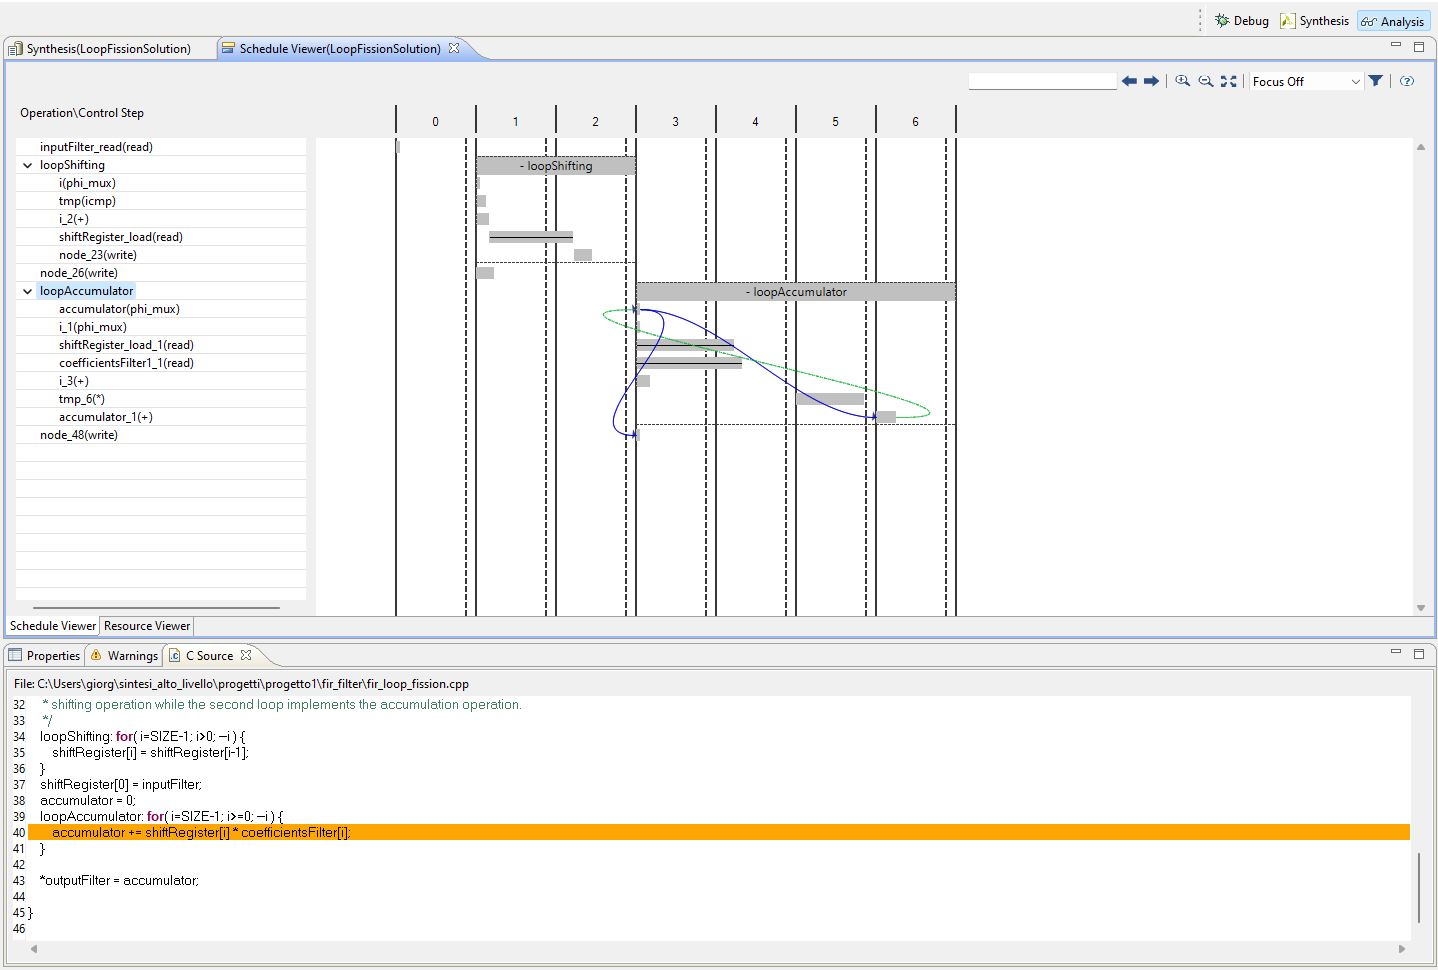
\includegraphics[width=1\textwidth]{solutions/loop_fission/loopfissionanalysis.png}
    \caption{HLS Loop Fission Solution Analysis}
\end{figure}

La scissione del loop nei cicli "loopShifting" e "loopAccumulator" la si può notare, inoltre, nella figura sopra allegata che mostra la finestra di \textit{Analysis}. Bisogna di nuovo precisare che, tale tecnica ha l'obiettivo di favorire l'ottimizzazione dei due loop in maniera indipendente effettuando magari uno scheduling delle operazioni differente, attraverso procedure proprietarie, rispetto alle soluzioni precedenti dove era previsto un unico ciclo for. 

\begin{table}[h]
    \centering
    \begin{tabular}{|l|c|c|c|c|}
        \hline
        \textbf{Name}    & \textbf{BRAM\_18K} & \textbf{DSP48E} & \textbf{FF} & \textbf{LUT} \\ \hline
        DSP              & -                   & -               & -           & -            \\ 
        Expression       & -                   & 2               & 0           & 96          \\ 
        FIFO             & -                   & -               & -           & -            \\ 
        Instance         & -                   & -               & -           & -            \\ 
        Memory           & 0                   & -               & 74          & 8            \\ 
        Multiplexer      & -                   & -               & -           & 110          \\ 
        Register         & -                   & -               & 131         & -            \\ \hline
        \textbf{Total}   & 0                   & 2               & 205         & 214          \\ \hline
        \textbf{Available} & 280               & 220             & 106400      & 53200        \\ \hline
        \textbf{Utilization (\%)} & 0            & $\sim$0               & $\sim$0     & $\sim$0      \\ \hline
    \end{tabular}
    \caption{HLS Loop Fission Solution Utilization Estimates Summary}
    \label{tab:hls-loop-fission-solution-utilization-estimates-summary}
\end{table}

\begin{table}[H]
    \centering
    \begin{tabular}{|c|c|c|c|c|c|c|c|}
        \hline
        \multicolumn{1}{|c|}{RTL} & \multicolumn{1}{|c|}{Status} & \multicolumn{3}{c|}{\textbf{Latency}} & \multicolumn{3}{c|}{\textbf{Interval}} \\
        &  & min & avg & max & min & avg & max \\
        \hline
        VHDL & Pass & 66 & 66 & 67 & 66 & 66 & 67 \\
        \hline
    \end{tabular}
    \caption{HLS Loop Fissiong Solution C/RTL Cosimulation Summary }
    \label{tab:hls-loop-fission-solution-cosimulation-summary}
\end{table}

\begin{table}[H]
    \centering
    \begin{minipage}[t]{0.45\linewidth}
        \centering
        \begin{tabular}{|l|r|}
            \hline
            \textbf{Resource} & \textbf{VHDL} \\
            \hline
            SLICE & 44 \\
            \hline
            LUT & 157 \\
            \hline
            FF & 106 \\
            \hline
            DSP & 2 \\
            \hline
            BRAM & 0 \\
            \hline
            SRL & 0 \\
            \hline
        \end{tabular}
        \caption{HLS Loop Fissiong Solution Export RTL Resource Usage}
        \label{tab:hls-loop-fission-solution-export-rtl-resoruce-usage}
    \end{minipage}
    \hfill
    \begin{minipage}[t]{0.45\linewidth}
        \centering
        \begin{tabular}{|l|r|}
            \hline
            \textbf{Timing} & \textbf{VHDL} \\
            \hline
            CP required & 10.000 \\
            \hline
            CP achieved post-synthesis & 5.745 \\
            \hline
            CP achieved post-implementation & 6.363 \\
            \hline
        \end{tabular}
        \caption{HLS Loop Fissiong Solution Export RTL Final Timing}
        \label{tab:hls-loop-fission-solution-export-rtl-final-timing}
    \end{minipage}
\end{table}

Si può evidenziare come, dopo aver effettuato l'Export RTL, il numero di cicli di clock affinché un risultato venga processato in uscita sia aumentato a 67 rispetto a quello ottenuto nella soluzione precedente pari a 43. Di fondamentale importanza è la diminuzione dell'utilizzazione delle risorse. Infatti, si può notare, rispetto alla soluzione hardware basata sul code hoisting, come il numero di SLICE sia diminuito di circa il $41\%$, quello delle LUT di circa il $42\%$ e quello dei FF di circa il $19\%$.
\\
Pertanto, importando l'IP in Vivado e impostando un clock constraint pari a 10ns è possibile analizzare i seguenti report di risorse, timing, potenza dinamica ed energia per singola operazione.
\lstinputlisting[language=VHDL]{solutions/loop_fission/clk_constraint.xdc}

\begin{table}[H]
    \centering
    \begin{tabular}{|c|c|c|c|c|c|c|}
        \hline
        \textbf{LUT} & \textbf{LUTRAM} & \textbf{FF} & \textbf{BRAM} & \textbf{DSP} & \textbf{IO} & \textbf{BUFG} \\
        \hline
        158 & 32 & 106 & 0 & 2 & 71 & 1 \\
        \hline
    \end{tabular}
    \caption{Vivado Loop Fission Solution Utilization Report [\#]}
    \label{tab:vivado-loop-fission-solution-utilization-reproot}
\end{table}

Si può notare come l'utilizzazione delle risorse sia minore ($-42\%$ LUT e $-21\%$ FF) rispetto alla solution precedente e, inoltre, la maximum clock frequency sia aumentata (dato dal fatto che il WNS è maggiore). Ovviamente, a tali vantaggi corrisponde, come già anticipato precedentemente, un aumento dei cicli di clock necessari ($+55.8\%$) affinchè un risultato venga processato in uscita.

\begin{table}[H]
    \centering
    \begin{tabular}{|c|c|c|c|}
        \hline
        \textbf{Cycles} [\#] & \textbf{Clock Constraint} [ns] & \textbf{WNS} [ns] & \textbf{Maximum Clock Frequency} [Mhz] \\
        \hline
        67 & 10 & 3.464 & 152.998776 \\
        \hline
    \end{tabular}
    \caption{Vivado Loop Fission Solution Timing Report}
    \label{tab:vivado-loop-fission-solution-timing-reproot}
\end{table}

\begin{table}[H]
    \centering
    \begin{tabular}{|c|c|c|c|c|c|c|}
        \hline
        \textbf{BRAM} & \textbf{Clock Enable} & \textbf{Clocks} & \textbf{DSP} & \textbf{Logic} & \textbf{Set/Reset} [mW] & \textbf{Data} \\
        \hline
        0 & 0.292603218 & 1.098937588 & 0.321194879 & 0.590288255 & 0.004160448 & 0.937705627 \\
        \hline
    \end{tabular}
    \caption{Vivado Loop Fission Solution Dynamic Power Report [mW]}
    \label{tab:vivado-loop-fission-solution-dynamic-power-reproot}
\end{table}

\begin{table}[H]
    \centering
    \begin{minipage}[t]{0.45\linewidth}
        \centering
        \begin{tabular}{|c|}
            \hline
            \textbf{Dynamic Total} \\
            \hline
            3.244890014 \\
            \hline
        \end{tabular}
        \caption{Vivado Loop Fission Solution Dynamic Power Report [mW]}
        \label{tab:vivado-loop-fission-solution-dynamic-power-reproot}
    \end{minipage}
    \hfill
    \centering
    \begin{minipage}[t]{0.45\linewidth}
        \centering
        \begin{tabular}{|c|}
            \hline
            \textbf{Energy Single Operation} \\
            \hline
            32.44890014 \\
            \hline
        \end{tabular}
        \caption{Vivado Loop Fission Solution Energy Single Operation Report [pJ]}
        \label{tab:vivado-loop-fission-solution-energy-single-operation-reproot}
    \end{minipage}
\end{table}

Si evidenzia che, la potenza dinamica totale e l'energia per singola operazione risultano essere diminuite, rispetto alla soluzione hardware precedente, di circa il $32\%$. In particolare, le maggiori diminuzioni si hanno in corrispondenza dei seguenti contributi: Clocks ($-38\%$), Logic ($-30\%$) e Data ($-32\%$). Infatti, bisogna ricordare che l'utilizzazione delle risorse, come già precedentemente citato, è anch'essa notevolmente diminuita rispetto alla solution precedente. 
